%----------------------------------------------------------------------------------------
%	PACKAGES AND THEMES
%----------------------------------------------------------------------------------------
\documentclass[aspectratio=169,xcolor=dvipsnames]{beamer}
\usetheme{SimplePlusAIC}

\usepackage{hyperref}
\usepackage{graphicx} % Allows including images
\usepackage{booktabs} % Allows the use of \toprule, \midrule and  \bottomrule in tables
\usepackage{svg} %allows using svg figures
\usepackage{tikz}
\usepackage{makecell}
\usepackage{epstopdf}
\newcommand*{\defeq}{\stackrel{\text{def}}{=}}
\usepackage{animate}
\usepackage{amsmath, amsthm, amscd, amsfonts, amssymb, graphicx, color}
\usepackage{mathtools,textcomp}
\usepackage[latin1]{inputenc}
\usepackage{amsmath,amssymb, mathrsfs}
\usepackage{minted}
\usepackage{listings}

\newcommand{\bm}{\boldsymbol}
\newcommand{\diff}{\operatorname{d}\!}
\newcommand{\tcolon}{\!:\!}

%Select the Epilogue font (requires luaLatex or XeLaTex compilers)
\usepackage{fontspec}
\setsansfont{Epilogue}[
    Path=./epilogueFont/,
    Scale=0.9,
    Extension = .ttf,
    UprightFont=*-Regular,
    BoldFont=*-Bold,
    ItalicFont=*-Italic,
    BoldItalicFont=*-BoldItalic
    ]

%----------------------------------------------------------------------------------------
%	TITLE PAGE
%----------------------------------------------------------------------------------------

\title[Portable Nonlinear Solid Mechanics Solver]{Performance-portable p-multigrid for nonlinear solid mechanics in nearly incompressible regime} % The short title appears at the bottom of every slide, the full title is only on the title page
%\subtitle{Subtitle}

\author[Surname]{Rezgar Shakeri, Jeremy L Thompson, and Jed Brown}
%\institute[CU Boulder]
% Your institution as it will appear on the bottom of every slide, maybe shorthand to save space


\date{\today} % Date, can be changed to a custom date
%----------------------------------------------------------------------------------------
%	PRESENTATION SLIDES
%----------------------------------------------------------------------------------------

\begin{document}

\begin{frame}[plain]
    % Print the title page as the first slide
    \titlepage
\end{frame}

%------------------------------------------------

\begin{frame}{Motivation}

\begin{minipage}{0.45\textwidth}
\textbf{Nonlinear Solver for Hyperelasticity}
{\large
    \begin{enumerate}
        \item Stable and reliable
        \item Efficient and accurate
        \item Compressible/Incompressible materials
    \end{enumerate}
}
\end{minipage}%	
\begin{minipage}{0.55\textwidth}
        \begin{figure}
            \includegraphics[width=0.85\linewidth]{figures/schwarz-mesh.png}
        \end{figure}
\end{minipage}

\end{frame}

%------------------------------------------------
\section{Stable Formulation- Single Field}
%------------------------------------------------

\begin{frame}{Standard Hyperelastic Formulation }

\textbf{Strong form}
{\Large
\begin{equation}
\nabla_X \cdot \bm{P} + \bm{f} = 0 \nonumber 
\end{equation}
}
where $\bm{P} = \bm{F} \bm{S}, \, \bm{F} = \bm{I} + \nabla_X \bm{u}, \, $ and for \textbf{Neo-Hookean Model}
{\Large
\begin{equation}
    \bm{S} = \frac{\lambda}{2} \left(J^2 - 1 \right) \bm{C}^{-1} + \mu \left(\bm{I} - \bm{C}^{-1} \right) \nonumber 
\end{equation}
}
where $J = \lvert \bm{F} \rvert, \, \bm{C} = \bm{F}^T \bm{F}, \,$ and $\lambda, \mu$ are Lame parameters.

\end{frame}

%------------------------------------------------

\begin{frame}[fragile]
\frametitle{Standard Hyperelastic Formulation}
    \begin{columns}[c] % The "c" option specifies centered vertical alignment while the "t" option is used for top vertical alignment
        \column{.4\textwidth} % Left column and width
        \begin{equation}
            \bm{S}(\nabla_X \bm{u}) = \frac{\lambda}{2} \left(J^2 - 1 \right) \bm{C}^{-1} + \mu \left(\bm{I} - \bm{C}^{-1} \right), \nonumber
        \end{equation}
        when $\nabla_X \bm{u} \ll 1 \Longrightarrow \bm{C} \approx \bm{I}, J \approx 1$

        \column{.6\textwidth} % Right column and width
        \begin{figure}
            \includegraphics[width=1.0\linewidth]{figures/unstable.png}
        \end{figure}
    \end{columns}
\vspace*{-20pt}
{\scriptsize
\begin{minted}{julia}
    function rel_error(eps, S, repr)
        ref = S(big.(eps*dudX)) 
        error = norm(S(repr.(eps*dudX)) - ref)
        error / norm(ref)
    end
\end{minted}
}      
\end{frame}

%------------------------------------------------
\begin{frame}{Stable Formulation}
    \begin{columns}[c] % The "c" option specifies centered vertical alignment while the "t" option is used for top vertical alignment

        \column{.4\textwidth} % Left column and width
        $\bm{C} = 2\bm{E} +  \bm{I} \Longrightarrow \bm{I} - \bm{C}^{-1} = 2 \bm{C}^{-1} \bm{E} $

        $$\bm{F} = \begin{bmatrix}
            1 + u_{0,0} & u_{0,1} \\
            u_{1,0} & 1 + u_{1,1}
        \end{bmatrix}$$
        $$J = 1 + (u_{0,0} + u_{1,1}) + u_{0,0} u_{1,1} - u_{0,1} u_{1,0} $$
        Stable compuation of $\mathtt{J_{-1}} = J - 1$ 
        $$\mathtt{J_{-1}} = u_{0,0} + u_{1,1} + u_{0,0} u_{1,1} - u_{0,1} u_{1,0} $$
        \textbf{Stable Neo-Hookean Model}
        \begin{equation}
            \bm{S} = \frac{\lambda}{2} \mathtt{J_{-1}} \left( \mathtt{J_{-1}} + 2 \right) \bm{C}^{-1} + 2 \mu \bm{C}^{-1} \bm{E} \nonumber 
        \end{equation}
        \column{.6\textwidth} % Right column and width

    \end{columns}

\end{frame}

%------------------------------------------------
\begin{frame}{Stable Formulation}
    \begin{columns}[c] % The "c" option specifies centered vertical alignment while the "t" option is used for top vertical alignment

        \column{.4\textwidth} % Left column and width
        $\bm{C} = 2\bm{E} +  \bm{I} \Longrightarrow \bm{I} - \bm{C}^{-1} = 2 \bm{C}^{-1} \bm{E} $

        $$\bm{F} = \begin{bmatrix}
            1 + u_{0,0} & u_{0,1} \\
            u_{1,0} & 1 + u_{1,1}
        \end{bmatrix}$$
        $$J = 1 + (u_{0,0} + u_{1,1}) + u_{0,0} u_{1,1} - u_{0,1} u_{1,0} $$
        Stable compuation of $\mathtt{J_{-1}}=J - 1$ 
        $$\mathtt{J_{-1}} = u_{0,0} + u_{1,1} + u_{0,0} u_{1,1} - u_{0,1} u_{1,0} $$
        \textbf{Stable Neo-Hookean Model}
        \begin{equation}
            \bm{S} = \frac{\lambda}{2} \mathtt{J_{-1}} \left( \mathtt{J_{-1}} + 2 \right) \bm{C}^{-1} + 2 \mu \bm{C}^{-1} \bm{E} \nonumber 
        \end{equation}
        \column{.6\textwidth} % Right column and width
        \begin{figure}
            \includegraphics[width=1.0\linewidth]{figures/stable-unstable.png}
        \end{figure}
    \end{columns}

% If we start with 8 digits number as an input, we cannot trust any digits of the output.
% Stable formulation is accurate for all-deformation elasticity. Important for mixed-precision Algorithm
\end{frame}

%------------------------------------------------
\section{Matrix Free}
%------------------------------------------------

\begin{frame}{Matrix Free}

\begin{itemize}
\item Modern hardware does 10 flops per byte.
\item Matrix-free methods store and move less data, compute faster.
\item The Jacobian of a non-linear operator rapidly loses the sparsity
\end{itemize}

\begin{align}
    \text{Residual:} \quad \bm{v}^T F(\bm{u}) &\sim \int_\Omega \bm{v} \cdot \color{olive}{f_0(\bm{u}, \nabla \bm{u})} + \color{black}{\nabla \bm{v}} \tcolon \color{olive}{f_1(\bm{u}, \nabla \bm{u})} \nonumber \\ 
    \text{Jacobian:} \quad \bm{v}^T J \diff \bm{u} &\sim \int_\Omega \begin{bmatrix} \bm{v} \\ \nabla \bm{v} \end{bmatrix}^T \color{teal}{\begin{bmatrix} f_{0,0} & f_{0,1} \\ f_{1,0} & f_{1,1} \end{bmatrix}}
    \begin{bmatrix} \diff \bm{u} \\ \nabla \diff \bm{u} \end{bmatrix} \nonumber
\end{align}

\end{frame}

%------------------------------------------------

\begin{frame}
\frametitle{Ratel: Extensible, Performance-Portable Solid Mechanics: {\href{https://gitlab.com/micromorph/ratel}{https://gitlab.com/micromorph/ratel}}}

\begin{figure}[H]
\hspace{-3mm}
    \includegraphics[width=1\textwidth]{figures/ratel-badge.png}
\end{figure}

\begin{minipage}{0.45\textwidth}
    \alert{\textbf{Features:}}
      \begin{itemize}
          \item Mixed/Linear elasticity
          \item Mixed/Neo-Hookean and Mooney-Rivlin Hyperelasticity
          \item Multi-material
          \item Static, Quasistatic, Dynamic
          \item Initial and Current configurations
      \end{itemize}
\end{minipage}%	
\begin{minipage}{0.55\textwidth}
    \begin{figure}
        \centering
        \includegraphics[width=0.9\textwidth]{figures/internal-api.png}
    \end{figure}
\end{minipage}

\end{frame}

%------------------------------------------------

\begin{frame}{\href{https://libceed.readthedocs.io}{libCEED}: Efficient Extensible Discretization}
\begin{figure}[t]
    \includegraphics[width=4in,height=1.6in]{figures/libCEEDAPI.png} % enter the filename here
\end{figure}

\begin{columns}[c] % The "c" option specifies centered vertical alignment while the "t" option is used for top vertical alignment

    \column{.5\textwidth} % Left column and width
    {\footnotesize
    \begin{itemize}
    \item \textcolor{red}{$\mathcal{P}$}: Process decomposition
    \item \textcolor{black}{$\mathcal{E}$}: Element restriction/assembly operator
    \item \textcolor{blue}{${B}$}: Basis (DoFs-to-Qpts) evaluator
    \item  \textcolor{green}{${D}$}: Operator at quadrature point- Qfunction
    \end{itemize}
    }
    \column{.5\textwidth} % Right column and width

    \end{columns}

\end{frame}

%------------------------------------------------

\begin{frame}{\href{https://libceed.readthedocs.io}{libCEED}: Efficient Extensible Discretization}
\begin{figure}[t]
    \includegraphics[width=4in,height=1.6in]{figures/libCEEDAPI.png} % enter the filename here
\end{figure}

\begin{columns}[c] % The "c" option specifies centered vertical alignment while the "t" option is used for top vertical alignment

    \column{.5\textwidth} % Left column and width
    {\footnotesize
    \begin{itemize}
    \item \textcolor{red}{$\mathcal{P}$}: Process decomposition
    \item \textcolor{black}{$\mathcal{E}$}: Element restriction/assembly operator
    \item \textcolor{blue}{${B}$}: Basis (DoFs-to-Qpts) evaluator
    \item  \textcolor{green}{${D}$}: Operator at quadrature point- Qfunction
    \end{itemize}
    }
    \column{.5\textwidth} % Right column and width
    {\footnotesize
    \begin{itemize}
    \item Purely algebraic high-order FEM Matrix-assembly and Matrix-free
    \item Single source Vanilla C for physics
    \item Various CPU and GPU backends with run-time selection \texttt{./bps -ceed /gpu/cuda}
    \end{itemize}
    }
    \end{columns}

\end{frame}

%---------------------------------------------------

\begin{frame}
    \frametitle{h-multigrid vs p-multigrid}
    \centering
    \includegraphics[height =0.8\textheight, width =0.55\linewidth]{figures/p-h-multigrid.png}

\end{frame}

%---------------------------------------------------

\begin{frame}
    \frametitle{p-multigrid}
    \begin{columns}[c] % The "c" option specifies centered vertical alignment while the "t" option is used for top vertical alignment
    \column{.4\textwidth} % Left column and width
    {\large
    \begin{itemize}
    \item 2nd order Chebyshev/Jacobi iteration in the range $[0.1\lambda_{max}, 1.1\lambda_{max}]$
    \item $\lambda_{max}$ estimate eigenvalue of $\left(\text{diag}\boldsymbol{A}_f \right)^{-1}\boldsymbol{A}_f$
    \item AMG use only information of the matrix sparsity and its entries of the assembled operators
    \end{itemize}
    }
    \column{.6\textwidth} % Right column and width
    \centering
    \includegraphics[width =0.95\linewidth]{figures/p-multigrid-cycle.png}
    \end{columns}

\end{frame}

%---------------------------------------------------

\begin{frame}
	\frametitle{Assembled vs Matrix-Free}
    \begin{columns}
        \column{0.4\linewidth}
        {\footnotesize
        \begin{itemize}
            \item Matrix-free becomes more efficient as the order increases
            \item Even for linear element, efficiency of matrix-free grows as DoFs increases since has smaller memory usage, thus achieves higher GDoF/s at the same memory bandwidth
            \item Both are latency-limited for smaller problem sizes (left of the figure) and the right is limited by memory bandwidth
        \end{itemize}
        }
        \column{0.6\linewidth}
        \centering
           \includegraphics[height =0.6\textheight]{figures/assemble-vs-matrixfree.png}
    \end{columns}
    \vspace*{-5pt}
    \centering
    \includegraphics[height =0.25\textheight, width =0.2\linewidth]{figures/schwarz-mesh.png}

\end{frame}

%------------------------------------------------
\section{Mixed-Elasticity}
%------------------------------------------------
\begin{frame}
\frametitle{Mixed-FE for Linear Incompressible Materials}
\begin{columns}
        \column{0.4\linewidth}
        {\Large
        \textbf{Strong Form}
        \begin{align}
            \nabla\cdot \bm{\sigma} + \bm{f} &= 0 \nonumber \\
            -\nabla\cdot\bm u -\frac{p}{\kappa} &=0 \nonumber
        \end{align}
        }
        where $\bm{\sigma} = -p \bm{I} + 2\mu \, \bm{\epsilon}_d$, $\bm{\epsilon}_d = \bm{\epsilon} - \frac{1}{3} \operatorname{trace} \left(\bm{\epsilon}\right) \, \bm{I}$, $ \bm{\epsilon} = \frac{1}{2} \left(\nabla\bm u +  \nabla\bm u ^T \right) $
        \column{0.6\linewidth}
        {\Large
        \textbf{Mixed-FE Form}
        \begin{equation} \nonumber
        \begin{bmatrix}
        \bm{A} & \bm{B}^T \\
        \bm{B} & \bm{C}
        \end{bmatrix}
        \begin{bmatrix}
        \bm{U}\\
        \bm{P}
        \end{bmatrix}
        = \begin{bmatrix}
        \bm{F}\\
        \bm{0}
        \end{bmatrix}
        \end{equation}
        }
        \begin{equation}
            \bm{A} \sim 2\mu \int_\Omega \nabla\bm{v}\,\bm{\epsilon}_d, \quad \bm{B} \sim -\int_\Omega q \, \nabla\cdot\bm{u} \nonumber 
        \end{equation}
        \begin{equation}
        \bm{C} \sim \frac{-1}{\kappa} \int_\Omega q \, p \nonumber 
        \end{equation}
    \end{columns}

\vspace*{20pt}

\textbf{Saddle point problem: When $\nu = 0.5 \Longrightarrow \bm{C} = 0 $.}

\end{frame}

%------------------------------------------------

\begin{frame}
\frametitle{Mixed-FE for Hyperelastic Materials}
\begin{columns}[c] 
    \column{.4\textwidth} % Left column and width
    {\Large
    \begin{align}
        \nabla_X \cdot \bm{P} + \bm{f} &= 0 \nonumber \\
        -\frac{1}{2 J} \left(J^2 - 1 \right) - \frac{p}{\kappa} &= 0 \nonumber
    \end{align}
    }

    \textbf{Standard Neo-Hookean Model}
    \begin{equation}
        \bm{S} = -p J \bm{C}^{-1} + \mu J^{-2/3} \left(\bm{C} - \frac{1}{3} \mathbb{{I}}_1(\bm{C}) \right) \bm{C}^{-1} \nonumber 
    \end{equation}
    \column{.6\textwidth} % Right column and width

    \end{columns}
\end{frame}

%------------------------------------------------

\begin{frame}
\frametitle{Mixed-FE for Hyperelasticty (Isochoric-Volumetric)}
\begin{columns}[c] 
    \column{.5\textwidth} % Left column and width
    {\Large
    \begin{align}
        \nabla_X \cdot \bm{P} + \bm{f} &= 0 \nonumber \\
        -\frac{\mathtt{J_{-1}}}{2 J} \left(\mathtt{J_{-1}} + 2 \right) - \frac{p}{\kappa} &= 0 \nonumber
    \end{align}
    }

    \textbf{Standard Neo-Hookean Model}
    \begin{equation}
        \bm{S} = -p J \bm{C}^{-1} + \mu J^{-2/3} \left(\bm{C} - \frac{1}{3} \mathbb{{I}}_1(\bm{C}) \right) \bm{C}^{-1} \nonumber 
    \end{equation}
    \textbf{Stable Neo-Hookean Model}
    \begin{equation}
        \bm{S} = -p J \bm{C}^{-1} + 2\mu J^{-2/3} \left(\bm{E} - \frac{1}{3} \mathbb{{I}}_1(\bm{E}) \right) \bm{C}^{-1} \nonumber 
    \end{equation}
    \column{.6\textwidth} % Right column and width
    \begin{figure}
            \includegraphics[width=0.95\linewidth]{figures/Iso-S.png}
    \end{figure}
    \end{columns}
\end{frame}

%------------------------------------------------

\begin{frame}
\frametitle{Inf-sup Constant $\beta$}
What would be the best choice for interpolation order of $\bm{u}, p$ ?
\vspace*{20pt}

\begin{figure}
\centering
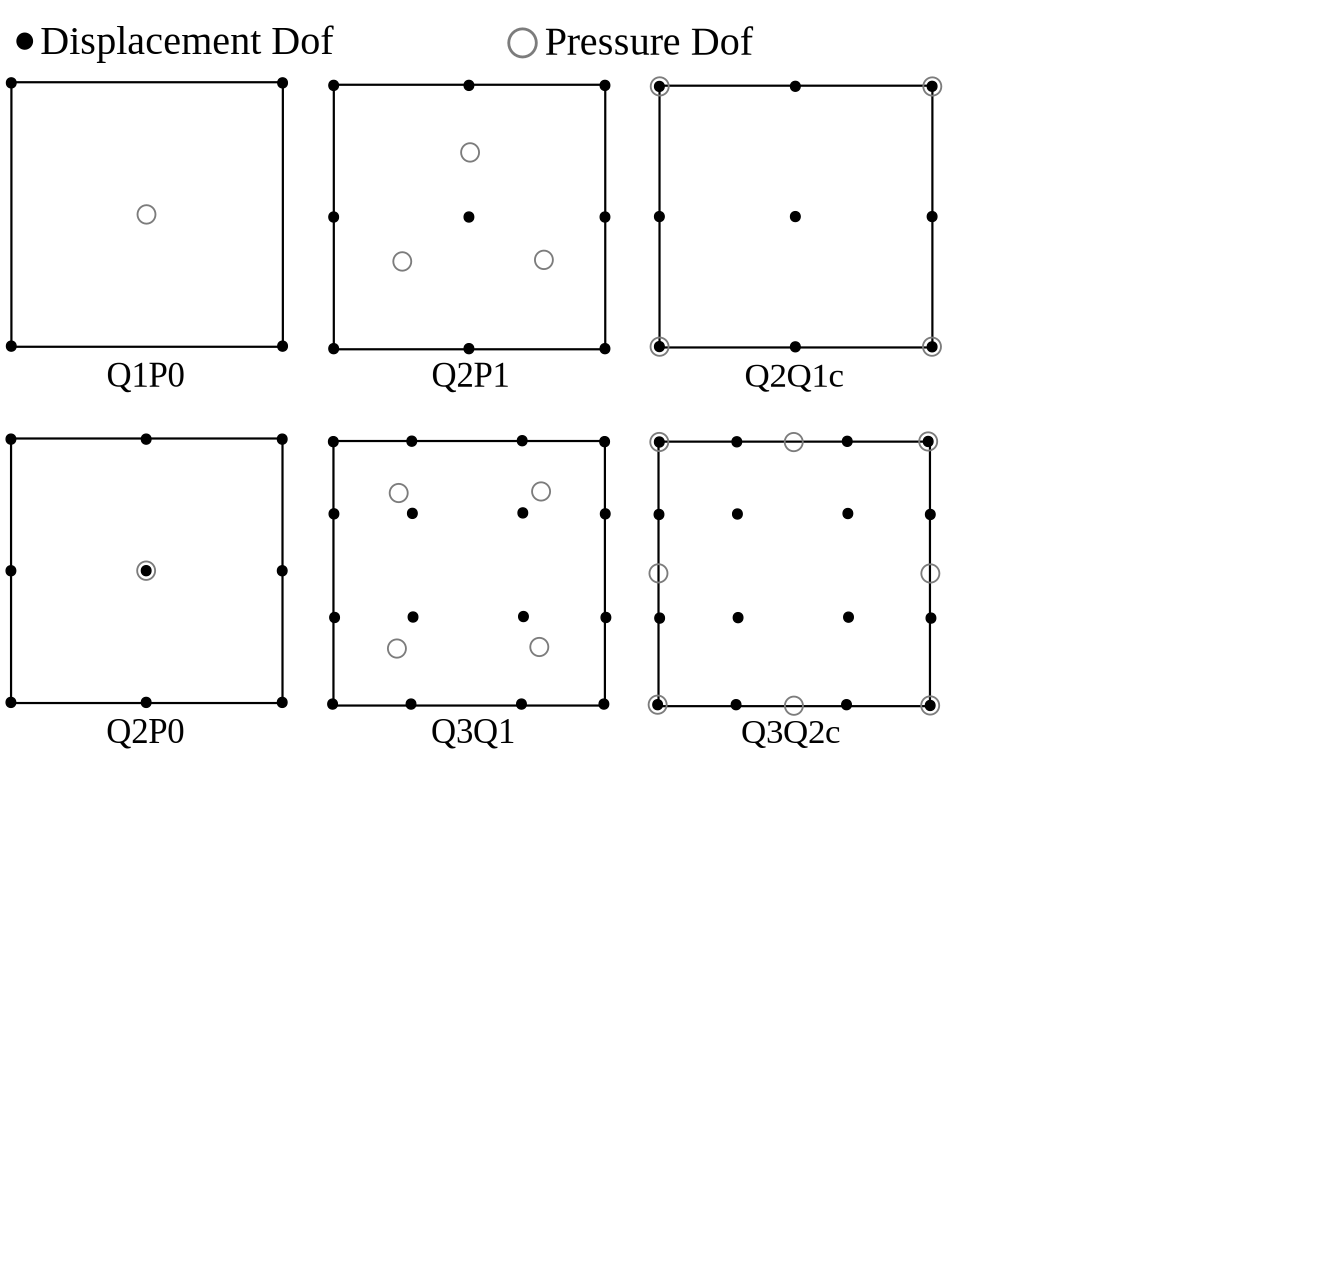
\includegraphics[width =1.5\textheight]{figures/mixed-element.png}
\end{figure}

\textbf{For $\bm{u}, \bm{v} \in \mathcal{V}$ and $p,q \in \mathcal{Q},$ solve:}
$$\langle\bm{u}, \bm{v} \rangle_{\mathcal{V}} + b(\bm{u},q) + b(\bm{v},p) = -\lambda \langle p, q \rangle_{\mathcal{Q}}, \qquad \beta = \sqrt{\lambda_{min}}, \qquad \beta \geq \beta_h >0 $$
        
\end{frame}

%------------------------------------------------

\begin{frame}
    \frametitle{Inf-sup Results for Discontinuous Pressure}
    \begin{columns}
        \column{0.5\linewidth}
        \centering
        \includegraphics[height =0.6\textheight]{figures/dist-p-1.png}
        \column{0.5\linewidth}
        %\centering
        %\includegraphics[height =0.6\textheight]{figures/dist-p-10.png}
    \end{columns}

\end{frame}

%------------------------------------------------

\begin{frame}
    \frametitle{Inf-sup Results for Discontinuous Pressure}
    \begin{columns}
        \column{0.5\linewidth}
        \centering
        \includegraphics[height =0.6\textheight]{figures/dist-p-1.png}
        \column{0.5\linewidth}
        \centering
        \includegraphics[height =0.6\textheight]{figures/dist-p-10.png}
    \end{columns}

\vspace*{5pt}
\begin{itemize}
    \item Q1P0, Q3Q2 are not stable.
    \item Stable element on uniform mesh may have issue on stretched case (Q2P1).
\end{itemize}

\end{frame}

%------------------------------------------------

\begin{frame}
    \frametitle{Inf-sup Results for Continuous Pressure}
    \begin{columns}
        \column{0.5\linewidth}
        \centering
        \includegraphics[height =0.6\textheight]{figures/cont-p-1.png}
        \column{0.5\linewidth}
        %\centering
        %\includegraphics[height =0.6\textheight]{figures/cont-p-10.png}
    \end{columns}

\end{frame}

%------------------------------------------------

\begin{frame}
    \frametitle{Inf-sup Results for Continuous Pressure}
    \begin{columns}
        \column{0.5\linewidth}
        \centering
        \includegraphics[height =0.6\textheight]{figures/cont-p-1.png}
        \column{0.5\linewidth}
        \centering
        \includegraphics[height =0.6\textheight]{figures/cont-p-10.png}
    \end{columns}
\vspace*{10pt}
\textbf{ All mixed elements with continuous pressure are inf-sup stable.}
\end{frame}

%------------------------------------------------

\begin{frame}
\frametitle{Conclusions and Outlook}	
\begin{itemize}
    \item Stable formulation for constitutive model is introduced for Neo-Hookean hyperelasticity and Isochoric-Volumetric split models.
    \item $\mathrm{H}^1$ mixed-FE is implemented in a matrix-free form.
    \item Inf-sup constants computed for all mixed elements with discontinuous/continuous pressure to determine unstable cases.
    \item We are developing a block preconditioner to have faster convergence for the mixed-form.
\end{itemize}

\end{frame}

%----------------------------------------------------------------------------------------
\end{document}